Comme présente la figure ~\ref{fig:scrum_process}, Scrum est un framework agile qui repose sur des cycles de développement appelés \textbf{sprints}. Chaque sprint a une durée définie (généralement entre 2 et 4 semaines) et aboutit à un produit fonctionnel et potentiellement livrable.
Le processus Scrum comprend plusieurs éléments clés :
\begin{itemize}
    \item \textbf{Product Backlog} : Liste des fonctionnalités à développer, priorisée par le Product Owner en fonction des besoins des utilisateurs et des objectifs du projet.
    \item \textbf{Sprint Backlog} : Ensemble des tâches à réaliser pendant un sprint, défini par l'équipe de développement.
    \item \textbf{Sprint Planning} : Réunion permettant de définir les objectifs et les tâches du sprint.
    \item \textbf{Daily Scrum} : Brève réunion quotidienne de l'équipe pour suivre l'avancement et identifier les obstacles.
    \item \textbf{Sprint Review} : Présentation de l'incrément produit aux parties prenantes à la fin de chaque sprint.
    \item \textbf{Sprint Retrospective} : Analyse du sprint pour identifier les axes d'amélioration.
\end{itemize}

\begin{figure}[H] % Use [H] to force the figure to appear exactly here
    \centering
    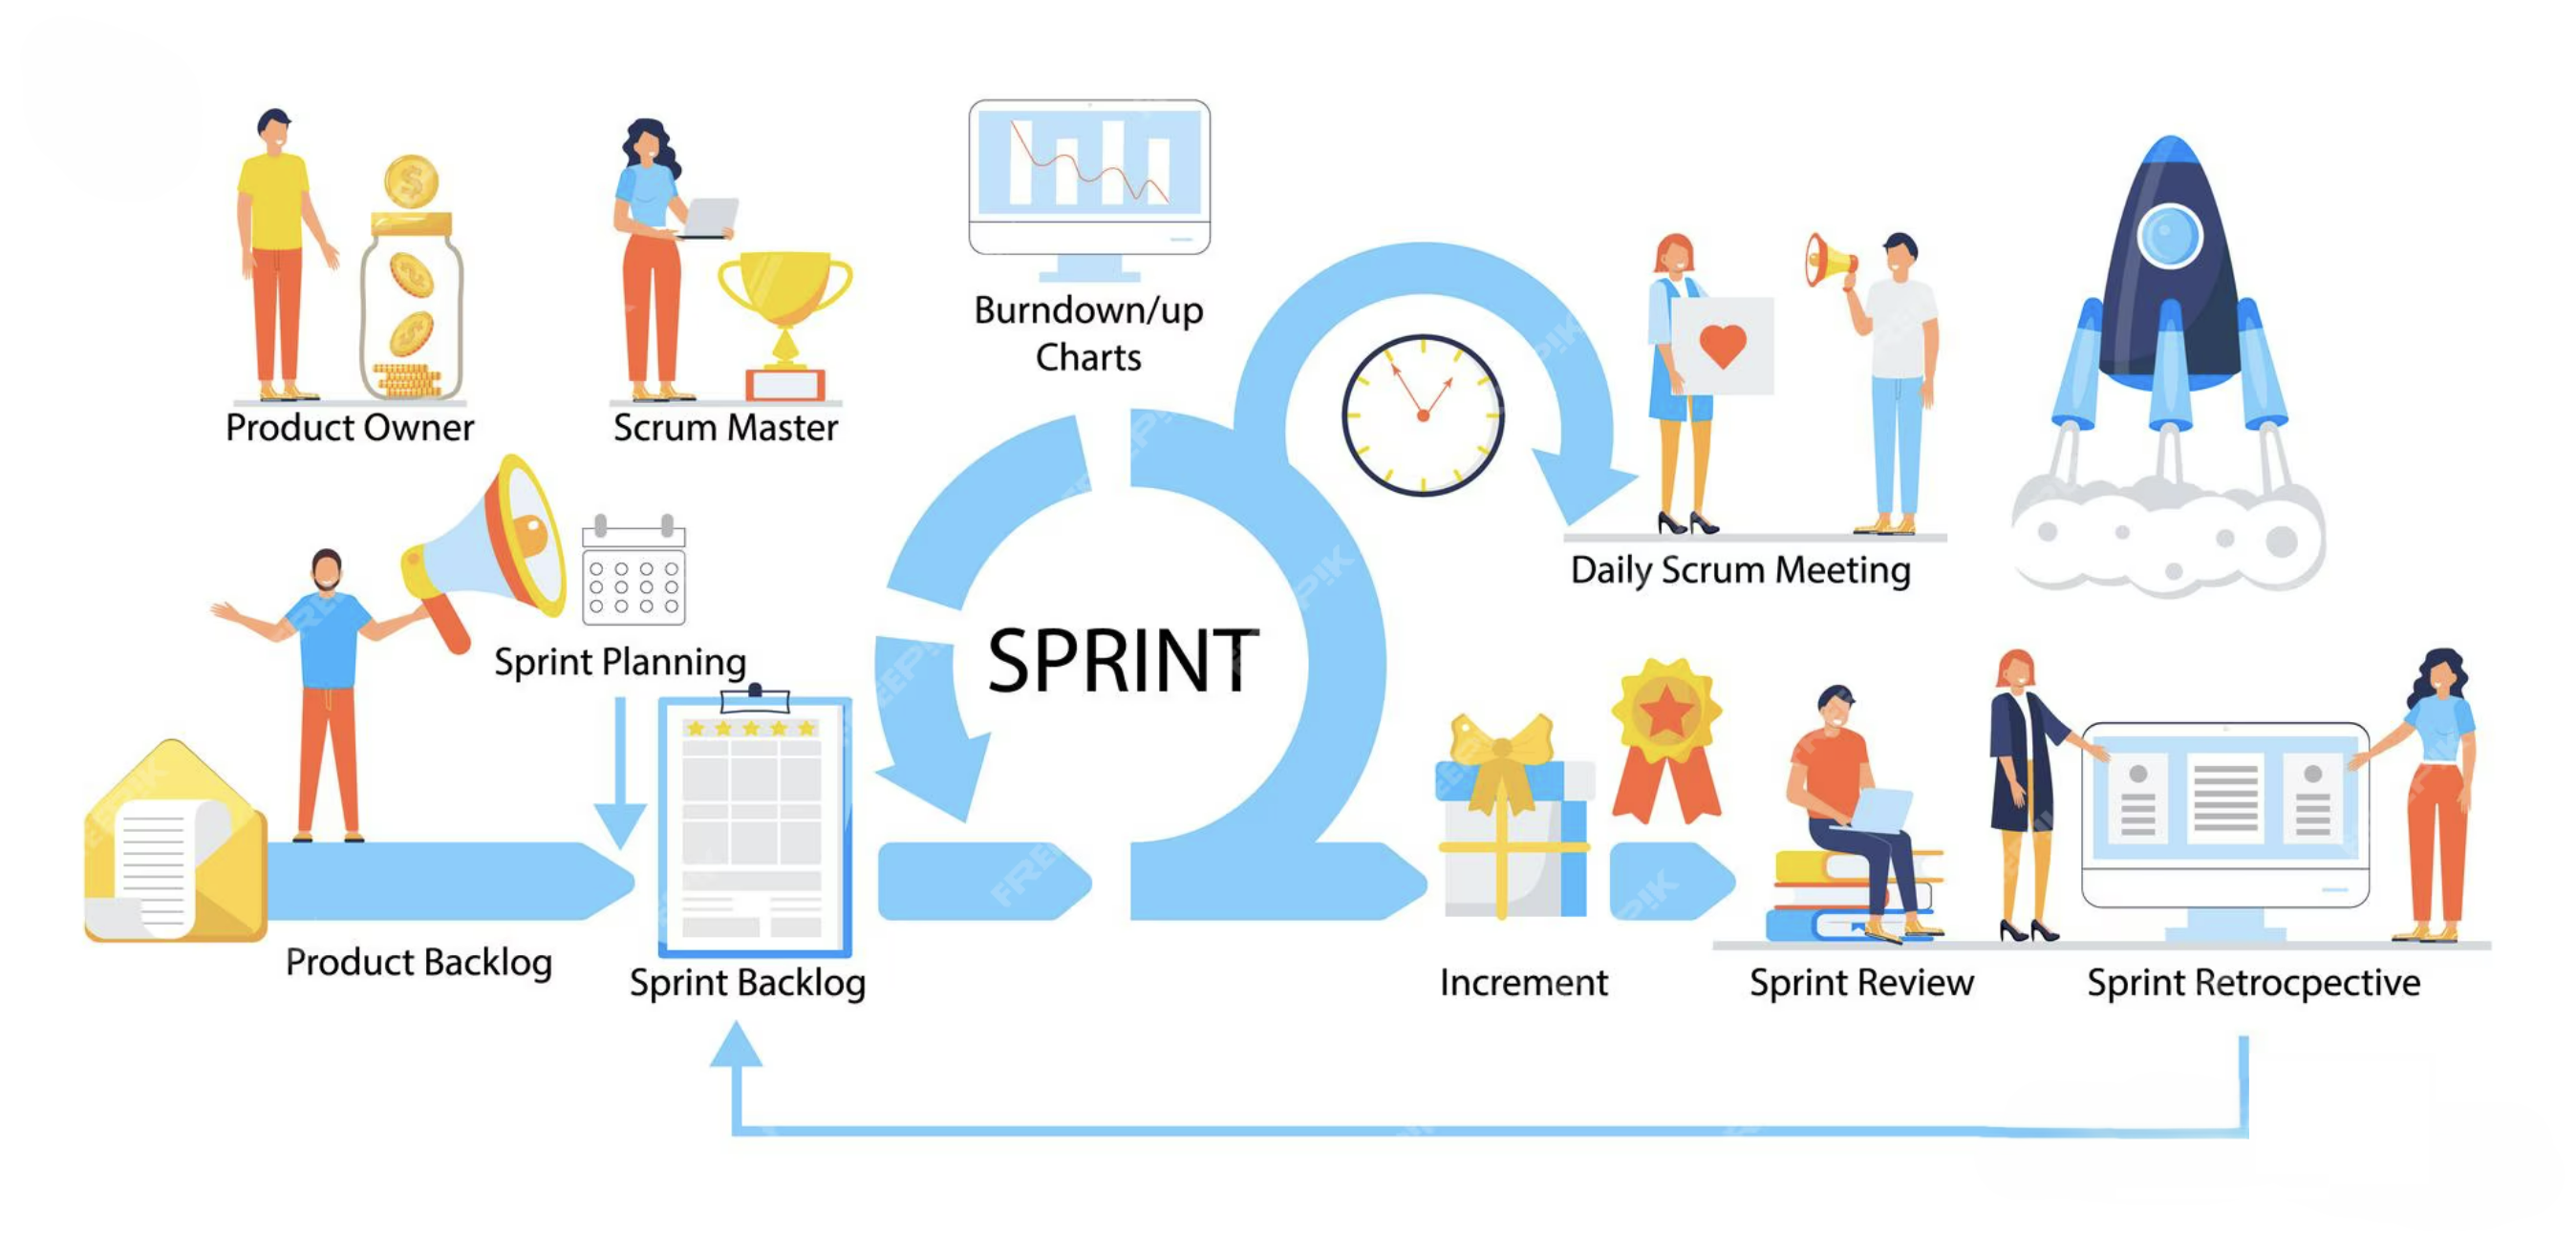
\includegraphics[width=1\linewidth]{chapter1/images/scrum.png} % Adjust width as needed
    \caption{Processus Scrum}
    \label{fig:scrum_process}
\end{figure}